\documentclass[11pt]{article}
% Shared preamble for main.tex, supplement1.tex and supplement2.tex
\setlength\parindent{10pt}
\usepackage{booktabs, amsmath, amssymb, mathrsfs, array, tabularx, makecell}
\usepackage[british]{babel}
\usepackage{csquotes}
% APA 7 references, as required by QSS at revision (compile with biber, e.g. latexmk)
\usepackage[style=apa, backend=biber, natbib=true]{biblatex}
\addbibresource{MyLibrary.bib}
\addbibresource{extra_refs.bib} % references not yet in Zotero
\usepackage[margin=1in]{geometry}
\usepackage{graphicx}
\usepackage{caption}
\usepackage{authblk} % author/affiliation management
\captionsetup[table]{skip=10pt}
\usepackage{tikz}
\usetikzlibrary{positioning, arrows.meta}
% Cross-references between the paper and its supplements: compile the
% supplements and the paper in turn (each reads the others' .aux files).
\usepackage{xr-hyper}
\usepackage{hyperref}
\pagestyle{plain}

\newcommand{\authorblock}{%
  \author[1]{Domingo Docampo}
  \author[2]{Lawrence Cram}
  \affil[1]{Atlantic Research Center for Information and Communication Technologies \newline University of Vigo, Vigo, Spain}
  \affil[2]{Research School of Physics, Australian National University, Canberra, 2600, ACT, Australia
  Charles Darwin University, Brinkin, 0810, NT, Australia}}
\newcommand{\papertitle}{Recirculating cardinal spectral ranking of journals and institutions}

\externaldocument[S1-]{supplement1}
\externaldocument[S2-]{supplement2}

\title{\papertitle}
\authorblock
\date{\today}

\begin{document}
\maketitle

\begin{abstract}
Bibliometric rankings usually treat journals and institutions differently, clouding
their inter-dependent roles.
We introduce a recirculating cardinal spectral ranking that treats journals and institutions
in four layouts:
journal to journal (similar to the Clarivate Eigenfactor score),
institution to institution (the institutional counterpart), all units to all units (full citation matrix),
and journal to institution to journal (recirculating or bipartite).
Stable, unique influence vectors for journals and institutions are derived by resolving
suitably conditioned matrix representations of these structures.
Applied to the economics and business journal literature in OpenAlex,
the method produces interpretable joint rankings with error bands, whose
sensitivity to model parameters is examined. The recirculating model
links journals and institutions to reinforce the hierarchy of influence. Journal influence agrees closely with the Article Influence Score, and departs from field-normalised citation scores in the direction of the standing of the citing units. Journal rankings are stabilised
by the inclusion of institutions, and very few units decline markedly over 25 years. The results also shed light on the relative standing of economics and business journals.
The study also uncovers enclaves, pockets of research in which hundreds of
highly cited works appear in low-ranked journals and come from low-ranked institutions.

\medskip\noindent
\textbf{Keywords}: spectral ranking, dual journal--institution influence,
Katz-Hubbell resolvent, ranking economics and business
\end{abstract}

% ---------------------------------------------------------------
\section{Introduction}
\label{sec:introduction}
% ---------------------------------------------------------------

The research system relies on journals and institutions. Journals filter
works through editorial and peer review, archive the literature, and
create metadata for retrieval and exploration. Institutions fund individual researchers,
implement training, oversee compliance, establish research organisational units
and maintain physical and information infrastructure. The influence hierarchy linking journals and institutions helps to shape the research system \citep{mertonSociologyScienceTheoretical1973, mcnameeStratificationScienceComparison1994, martinTiedKnowledgePower1998}, yet studies that treat journals and institutions symmetrically are infrequent. More commonly, the hierarchy of journals is established first, perhaps by spectral ranking, and the institutional hierarchy is derived from it by aggregation. It is therefore unknown whether institutional spectral rankings yield useful orderings, and how joint ranking changes rankings of either component. This paper proposes a cardinal spectral ranking of journals and institutions treated in parallel, revealing how the recursive exchange of references between research articles helps to form and maintain influence. 

The introduction of the science citation index \citep{garfieldScienceCitationIndex1964} facilitated the exploration of connections between journals and institutions by `inverting' the reference list of each work back to a convenient index of citing works and their targets \citep{woutersCitationCulture1999}. Citation-based journal ranking immediately became a useful means to manage collections and to select outlets for publications. On the other hand, the rapid and widespread misuse of the journal impact factor (JIF) as proxy for the importance of research works exemplified tensions in bibliometric evaluation that remain unresolved \citep{garfieldCitationAnalysisLegitimate1979,bornmannCitationCountsResearch2008, leydesdorffCitationsIndicatorsQuality2016, macrobertsMismeasureScienceCitation2018}. Perhaps due to the complexity of institutions' disciplines and missions, an institution impact factor (IIF) has not emerged. Rather, institutional rankings derived from bibliometric indicators of works, authors or journals are often composed with other indicators to form an institutional score. This is the approach in global rankings such as QS, Times Higher Education (THE), Shanghai (ARWU), Leiden Ranking (CWTS) and SCImago Institutions Rankings, as well as many national performance-based research funding schemes \citep{zacharewiczPerformancebasedResearchFunding2019}. 

There are hundreds of algorithms for extracting information from a citation index. For example, \textcite{pendleburyUseMisuseJournal2009} presents a critical survey of around a dozen journal rankings, while \textcite{kanellosImpactbasedRankingScientific2019} present a critical comparative study of more than 30 methods for ranking articles over the work-work citation network. \textcite{adlerCitationStatisticsReport2009} [see also \textcite{lehmannCommentCitationStatistics2009}] offer cautionary advice about these algorithms in general. Their report comments on a `mystical belief in the magic of citation statistics' and reserves a special mention for the eigenvector methods studied in this paper: `Their proponents make claims about their efficacy that are unjustified by the analysis and difficult to assess. Because they are based on more complicated calculations, the (often hidden) assumptions behind them are not easy for most people to discern.' Mindful of this evaluation, we find the calculations uncomplicated, aim to reveal our assumptions and parameters, attach error bands to every influence value, and test agreement with established indicators, reporting where and why they disagree.

The spectral methods explored in this paper can be traced to studies of recursive methods for computing centrality in social networks \citep{vignaSpectralRanking2016}, although these were 
not referenced by \textcite{narinEvaluativeBibliometricsUse1976}, \textcite{pinskiCitationInfluenceJournal1976}, and \textcite{narinStructureBiomedicalLiterature1976} when they proposed a recursive method to construct influence weights of journals within a disciplinary field. To obtain influence weights for institutions, Narin et al. aggregated the institutional publications in a field weighted by the respective journal influence score. Over a sample of several dozen universities, the total institution influence scores were well-correlated with survey-based rankings, but also with the number of publications, suggesting that survey respondents combined influence and size. Narin's work developed into the eigenvector approach now widely used for journal ranking \citep{bollenJournalStatus2006, bergstromEigenfactorMetrics2008, franceschetTenGoodReasons2010, vignaSpectralRanking2016}. 

Eigenvector methods have been also applied to author-level influence weightings in the field of social science by \textcite{westAuthorlevelEigenfactorMetrics2013}. This work extended Narin's aggregation approach to ranking institutions and countries, and appended an exploration of spectral ranking over distinct kinds of entities that anticipates the approach taken here. An alternative approach iterates between the article-article network and the corresponding article-author network \citep{ujumBestBothWorlds2015, palCITEXNewCitation2015}. \textcite{chenArticlesScientificPrestige2023} present an extensive comparison, within topic clusters, between (a) PageRank ranking over the article reference network and (b) the articles' simple citation count. The formulation by \textcite{caoRankingAcademicInstitutions2023} considers the article-article and article-institution network, ranked by a novel and effective iteration over random walks. This is one of the few reported spectral rankings of institutions. The authors note that a limiting case of their approach corresponds to the eigenvector (PageRank) method, while \textcite{gellerCitationInfluenceMethodology1978} noted earlier that random walks over Markov chains are closely related to the spectral ranking introduced by Narin et al. 

We foreground our choice to view references and citations through the lens of Social Systems Citation Theory \citep[][SSCT]{tahamtanSocialSystemsCitation2022}. It concentrates on the structural features of the network of references and citations, setting aside authorial, editorial and managerial intent. This approach contrasts with actor-network theory \citep[][ANT]{latourReassemblingSocialIntroduction2007}, which foregrounds the intentful roles of heterogeneous agents including authors
in assembling citation networks. ANT will be important in our follow-up studies that relate this paper to the referencing activities of individual researchers, such as the `enclaves' featured in the Discussion. Note also that in the face of potential confusion around the words `reference' and `citation', we prefer `reference.' We say work $w_1$ references a work $w_2$ in its reference list and, if necessary, that $w_2$ is cited by $w_1$ \citep{woutersCitationCulture1999}.

The paper proceeds as follows. The next section summarises the model: journal and institution units coupled by the reference lists of the works they publish, and the steady-state distribution of influence among them. Supplement~1 gives the full mathematical framework and the numerical methods. We then construct a corpus of works in the fields of economics and business, describe how its metadata errors are corrected and measured, and form subsets of the corpus to illustrate the interconnections of units, subfields, and time. We present spectral rankings over these subsets, alongside sensitivity studies of the key parameters and a summary of the error studies reported in Supplement~2. We compare journal influence with the Article Influence Score, and journal and institution influence with field-normalised citation scores computed on the same corpus. The findings are applied to help explain ranking differences between the broad fields of economics and business, and to identify enclaves of highly cited work in low-ranking units. The paper discusses these results including a critique of our methods, and concludes with some directions for future work.


%!TeX root = ../main.tex
% ---------------------------------------------------------------
\section{The model in brief}
\label{sec:networks}
% ---------------------------------------------------------------

This section summarises the model; Supplement~1 gives the full framework, the derivations and the numerical methods, and its Table~\ref{S1-tab:notation} lists the notation.

The units of the model are journals (OpenAlex sources, $S$) and institutions ($I$), and both are nodes of one network. Every work in the corpus has one journal and one or more institutions. A work's institution weights $\omega_{iu}$ sum to one: each author carries an equal share of the work, divided equally among the author's institutions (author-fractional counting, $\omega=0$). The work count $a_p$ of a unit $p$ is the number of its works, counted in the same fractional way for institutions.

When work $w_i$ includes work $w_j$ in its reference list, the reference is read as a flow of attention from the units of $w_i$ to the units of $w_j$ (Figure~\ref{fig:schematic}). Summed over all corpus references, these flows form a unit-by-unit reference matrix $\mathbf{C}$ with four blocks: journal to journal ($\mathbf{C}_{SS}$), journal to institution ($\mathbf{C}_{SI}$), institution to journal ($\mathbf{C}_{IS}$) and institution to institution ($\mathbf{C}_{II}$). Rows index the referencing unit and columns the referenced unit, so a row sum counts references given and a column sum counts citations received. Each reference of $w_i$ is weighted by $\bar{R}/R_i$, where $R_i$ is the number of corpus references of $w_i$ and $\bar{R}$ is their mean, so that every reference list carries the same total weight ($\rho=0$).

\begin{figure}[!htb]
  \centering
  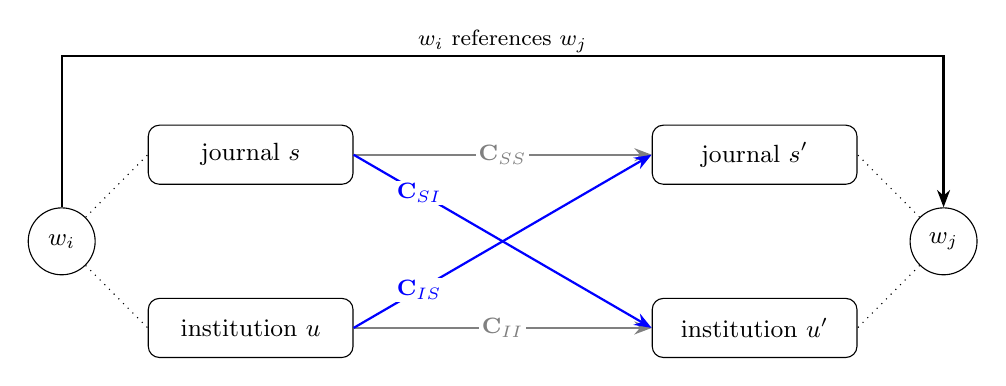
\begin{tikzpicture}[
      unit/.style={draw, rounded corners, minimum width=2.6cm, minimum height=0.75cm, font=\small},
      work/.style={draw, circle, minimum size=0.85cm, font=\small},
      flow/.style={-{Stealth[length=2.2mm]}, thick},
      lab/.style={font=\footnotesize, fill=white, inner sep=1pt}]
    \node[unit] (s)  at (0, 1.1)  {journal $s$};
    \node[unit] (u)  at (0,-1.1)  {institution $u$};
    \node[unit] (s2) at (6.4, 1.1) {journal $s'$};
    \node[unit] (u2) at (6.4,-1.1) {institution $u'$};
    \node[work] (wi) at (-2.4, 0) {$w_i$};
    \node[work] (wj) at (8.8, 0)  {$w_j$};
    \draw[dotted] (wi) -- (s.west);  \draw[dotted] (wi) -- (u.west);
    \draw[dotted] (wj) -- (s2.east); \draw[dotted] (wj) -- (u2.east);
    \draw[flow] (wi) |- (3.2, 2.35) node[lab, above] {$w_i$ references $w_j$} -| (wj);
    \draw[flow, gray] (s) -- node[lab, pos=0.5] {$\mathbf{C}_{SS}$} (s2);
    \draw[flow, gray] (u) -- node[lab, pos=0.5] {$\mathbf{C}_{II}$} (u2);
    \draw[flow, blue] (s.east) -- node[lab, pos=0.22] {$\mathbf{C}_{SI}$} (u2.west);
    \draw[flow, blue] (u.east) -- node[lab, pos=0.22] {$\mathbf{C}_{IS}$} (s2.west);
  \end{tikzpicture}
  \caption{A reference from work $w_i$ to work $w_j$ is projected onto the units that publish the two works (dotted). It adds weight to the four blocks of the reference matrix: journal to journal ($\mathbf{C}_{SS}$), institution to institution ($\mathbf{C}_{II}$), and the cross blocks $\mathbf{C}_{SI}$ and $\mathbf{C}_{IS}$ (blue). The bipartite baseline uses only the cross blocks, so influence circulates journal $\to$ institution $\to$ journal. A work with several institutions spreads its weight over them by author-fractional counting.}
  \label{fig:schematic}
\end{figure}

A binary mask $\mathbf{m}=(m_{SS},m_{SI},m_{IS},m_{II})$ selects the blocks that enter the ranking. It gives four layouts: journal-only ($1000$), institution-only ($0001$), full joint ($1111$) and bipartite ($0110$). The journal-only layout is close to the construction of the Eigenfactor and Article Influence Score \citep{bergstromEigenfactorMetrics2008}, and the institution-only layout is its institutional counterpart. In the bipartite layout, our baseline, influence passes only from journals to institutions and back. A journal gains influence when its works are referenced by works from influential institutions, and an institution gains influence when its works are referenced by works in influential journals. In the joint and bipartite layouts the weight $\chi$ balances the journal and institution sides ($\chi=0.5$).

Each row of the masked matrix is normalised to sum to one, giving a Markov transition matrix $\mathbf{H}$. The ranking probability $\boldsymbol{\pi}$ is its stationary distribution, the Perron--Frobenius eigenvector $\mathbf{H}^\top\boldsymbol{\pi}=\boldsymbol{\pi}$ with $\mathbf{1}^\top\boldsymbol{\pi}=1$ \citep{pinskiCitationInfluenceJournal1976, gellerCitationInfluenceMethodology1978}. Supplement~1 also gives the Katz--Hubbell generalisation with attenuation $\alpha<1$ and prior $\boldsymbol{\mu}$, which we use only as a sensitivity check. The reported quantity is the \emph{influence} per work \citep{palacios-huertaMeasurementIntellectualInfluence2004},
\begin{equation}
  v_p \;=\; \frac{A\,\pi_p}{a_p}, \qquad A=\sum_p a_p .
  \label{eq:vstar}
\end{equation}
The $a$-weighted mean of $v$ is one, so $v$ is a ratio scale \citep{stevensTheoryScalesMeasurement1946}: $v=1$ is the corpus-average influence per work and $v=2$ twice that. It is the counterpart of influence per publication \citep{pinskiCitationInfluenceJournal1976} and of the Article Influence Score. A unit's total influence is proportional to $\pi_p=a_p v_p/A$. Table~\ref{tab:parameters} lists the parameters and their baseline values.

\begin{table}[!bt]
  \centering
  \caption{Model parameters and baseline values.}
  \label{tab:parameters}
  \renewcommand{\arraystretch}{1.00}
  \begin{tabularx}{\textwidth}{@{}cXc@{}}
    \hline
    Parameter & Description & Baseline \\
    \hline
    \multicolumn{3}{@{}l}{\textit{Corpus construction}} \\[2pt]
    $\tau_S$ & Threshold works/journal/year & 10 \\
    $\tau_I$ & Threshold works/institution/year & 20 \\
    $F$      & Fields: $E$ (economics), $B$ (business), $A$ (ambiguous),
               $X$ (none) & $EBAX$ \\
    $t_c$    & Census window: publication years of referencing works & 2020--2024 \\
    $t_t$    & Target window: publication years of referenced works & 2020--2024 \\[4pt]
    \multicolumn{3}{@{}l}{\textit{Reference matrix assembly}} \\[2pt]
    $\rho$   & Reference-list weights: $\rho=0$, normalise by $\bar{R}/R_i$; $\rho=1$, raw counts & 0 \\
    $\omega$ & Institution weights: $\omega=0$, author-fractional; $\omega=1$, equal shares $1/n_i$ & 0 \\
    $\mathbf{m}$ & Block mask: $1000$ journal-only, $0001$ institution-only,
               $1111$ joint, $0110$ bipartite & 0110 \\
    $\chi$   & Journal--institution mixing weight: $\chi=0.5$ or $\chi^*=N_I/(N_S+N_I)$ & 0.5 \\
    $\varepsilon$ & Sentinel flag: $\varepsilon=0$, within-corpus only;
               $\varepsilon=1$, include sentinel units & 0 \\[4pt]
    \multicolumn{3}{@{}l}{\textit{Resolvent}} \\[2pt]
    $\alpha$ & Attenuation: $\alpha=1$, Perron--Frobenius; $\alpha<1$, Katz--Hubbell & 1 \\
    $\mu$    & Prior with $\alpha<1$: uniform $1/(N_S+N_I)$, or $1/2N_S$ and $1/2N_I$ & n.a. \\
    \hline
  \end{tabularx}
\end{table}

%!TeX root = ../main.tex
% ---------------------------------------------------------------% ---------------------------------------------------------------
\section{Corpus selection}
\label{sec:sources}
OpenAlex \citep{priemOpenAlexFullyopenIndex2022, alperinAnalysisSuitabilityOpenAlex2024, vaneckneesjanOpeningCWTSLeiden2024} provides our bibliometric data. We select the fields of economics and business due to their traditions of evaluative ranking of journals and institutions \citep[e.g.][]{liebowitzAssessingRelativeImpacts1984, boricPossibilitiesRankingBusiness2024}. Corpus selection starts with a list of eligible sources having three features: evidence from one of our journal registries that the source substantially 
publishes economics or business research, an OpenAlex source identifier for corpus extraction, and a sufficient number of published works per year.

The journal registries are as follows. Harzing's \textit{71st Edition of the Journal Quality List}~\textcite[][JQL]{harzingJournalQualityList2024} assembles
peer assessments of journal quality across business and economics
disciplines. Its scope is confined to economics and business so no
filtering is applied.
The \textit{ERA 2023 Submission Journal List}~\textcite[][SJL]{australianresearchcouncilERA2023Submission2022} assigns up to three
Field of Research (FoR) codes to each entry.
From the full list of 26{,}241 journals we retain those for which \emph{every} assigned FoR code falls within
Division~35 (Commerce, Management, Tourism and Services) or
Division~38 (Economics)---specifically the 35 and 38 two-digit divisions and the four-digit groups
3501--3509 and 3801--3803, 3899.
\textit{Clarivate Web of Science Journal Citation Reports}~\textcite[][JCR]{clarivateanalyticsJournalCitationReports2026} assign each
journal a Web of Science category. We retain those in
``Economics'', ``Management'', ``Business'', ``Transportation'',
or ``Business, Finance''.
The \textit{Scopus Source List}~\textcite[][SSL]{elsevierScopusSourceList2026} (March 2026 edition) assigns All Science Journal Classification (ASJC) codes to each source. We retain journals carrying code~1400 (Business, Management and Accounting) or code~2000 (Economics, Econometrics and Finance), including inactive titles.

Every journal in JQL, SJL, JCR, and SSL has at least one ISSN, and may have several. These registry ISSNs are joined independently to the February 2026 OpenAlex sources snapshot using its list of ISSNs as the matching key and selecting only the `journal' source-type. Around 60 additional matches are identified by exact title matching for OpenAlex sources that lack an ISSN. We denote the union of matched OpenAlex sources OAS\textsuperscript{**}. Some of these sources publish mainly in fields such as sociology, psychology, technology, education or law. Using the OpenAlex topic/field entity, we drop sources with less than 40\% of their OpenAlex assigned field count in \textit{Economics, Econometrics, and Finance} or \textit{Business, Management and Accounting}. We denote the remaining sources OAS\textsuperscript{*}.

Once the OAS\textsuperscript{*} sources list is established, we conduct a preliminary extract of work and authorship data to identify sources or institutions with few works over the period 2020-2024. Sorting sources by their works count, the relation between total dropped works and sources leads us to retain sources that publish on average $\tau_S \ge 10$ works/source/year. Sources retained above the threshold $\tau_S$ form the set OAS. Following the same steps for institutions, we truncate the long tail of low-output institutions by adopting a threshold of $\tau_I \ge 20$ works/institution/year. Many of the institutions removed at this point are fragments of larger institutions not blended by OpenAlex, or technology-focussed institutions with a small output of business scholarship. 

Selecting sources and institutions that satisfy these thresholds, we extract works, authorships and reference lists published between 2000 and 2024, retaining works typed as article or review, and excluding works that are paratext, retracted, or without an authorship entity. We retain institutions from a work's authorship metadata if the OpenAlex institution type is education, nonprofit, government, or other, while excluding companies and funders. Although most results relate to the recent 5-year window 2020-2024, we choose the wider 2000--2024 time window to support our time-series and error analyses.

\begin{table}[!htbp]
\centering
\caption{Registry and OpenAlex sources classified by field $E/B/A/X$. The upper section counts each appearance in a registry and field. JQL: Harzing Journal Quality List; JCR: Web of Science Journal Citation List; SJL: ERA Subject Journal List; SSL: Scopus Source List. OAS$^{**}$ is the union of all registry sources matched to OpenAlex. OAS$^{*}$ drops sources whose OpenAlex topic content is less than 40\% economics or business. OAS drops sources publishing at a rate below $\tau_S$.}
\label{tab:registry_overview}
\begin{tabular}{lrrrrrrrr}
\toprule
Registry & Sources & OA Match & Match\% & E & B & A & X \\
\midrule
JQL & 850 & 836 & 98.4\% & 233 & 377 & 33 & 193 \\
JCR & 1,433 & 1,397 & 97.5\% & 555 & 674 & 83 & 85 \\
SJL & 1,624 & 1,381 & 85.0\% & 417 & 806 & 75 & 83 \\
SSL & 2,983 & 2,770 & 92.9\% & 745 & 1,072 & 238 & 715 \\
\midrule
OAS$^{**}$ & 3,534 & --- & --- & 860 & 1,306 & 295 & 1,073 \\
OAS$^{*}$ & 2,121 & --- & --- & 764 & 1,058 & 203 & 95 \\
OAS & 1,693 & --- & --- & 613 & 855 & 154 & 71 \\
\bottomrule
\end{tabular}
\end{table}

Within the broad field of Economics and Business, many sources publish works in smaller subfields $F$ within the set $\mathfrak{F}$. To relate OAS sources to subfields ${F}$ we capitalise on registry subfield labels (categories, groups, subjects, ASJC and topics in JQL, SJL, JCR, SSL, and OAS respectively). These labels are mapped by hand to the broad subfields $F=E$ (economics) or $F=B$ (business), or $F=X$ when the subfield is out of scope (e.g. Psychology, Education from JQL). Some sources publish across $E$ and $B$; they are designated ambiguous, $F=A$. The five signals are counted, and each source classified according to this sequence:
\begin{itemize}
	\setlength{\itemsep}{0pt}
	\item `X' when $E$-count + $B$-count $< 2$ (weak in both fields);
	\item `A' $E$-count = $B$-count (ambiguous);
	\item `E' $E$-count $>$ $B$-count (economics-dominant);
	\item `B' $B$-count $>$ $E$-count (business-dominant).
\end{itemize}
Finally, a source classified `E' or `A' is reclassified `B' if at least two of four registry signals mark it as finance or accounting (JQL `F\&A', JCR `Business, Finance', SJL codes 3501 or 3502, OpenAlex subfield Finance or Accounting), since these fields are usually anchored in business schools. A single signal is not sufficient: SJL code 3502 is a secondary code for many economics journals. Four economics journals that meet the two-signal rule are kept in $E$ (\textit{Journal of Monetary Economics}, \textit{Fiscal Studies}, \textit{IMF Economic Review}, \textit{Intereconomics}). Of the 1,564 baseline sources, 525 are classified $E$, 876 $B$, 101 $A$ and 62 $X$.
Table~\ref{tab:registry_overview} summarises the number of matched sources in the registries by field, and indicates the effects of removing sources predominantly outside economics and business, or publishing few works in 2020-2024. 

Institutions often host both business and economics, and direct categorical classification is problematic. 
To indicate the balance of $E$ and $B$ for an institution
we use the stochastic reference matrix $H_{SI}$ to relate an institution to already-classified sources. For each source~$s$, $H_{SI}[s,u]$ is the fraction of $s$'s reference weight directed at institution~$u$. 
The sum over sources in field $F$, $f_{Fu}$, is the fraction of institution~$u$'s incoming reference weight from $F$-classified sources. These fractions are sorted and institutions assigned field labels by a quota rule matched to the field-distribution of sources: top 30\% by $f_{Xu}$ receive $X$; from the remainder, top 10\% by $f_{Au}$ receive $A$; of the rest, institutions with $f_{Eu}\geq f_{Bu}$ receive $E$ (up to a 5:8 $E$:$B$ quota, which does not bind) and the others $B$. Classification of institutions by subfield describes no more than tendency.


\begin{table}[!bt]
  \centering
  \caption{Glossary.}
  \label{tab:parameters}
  \renewcommand{\arraystretch}{1.00} %1.25}
  \begin{tabular}{@{}clcc@{}}
    \hline
    Parameter & Description & Baseline \\
    \hline
    \multicolumn{3}{@{}l}{\textit{Corpus construction}} \\[2pt]
    $\tau_S$ & Threshold works/source/year & 10 \\
    $\tau_I$ & Threshold works/institution/year & 20 \\
    $F$      & Fields: $E$ (economics), $B$ (business), $A$ (ambiguous),
               $X$ (none) & $EBAX$ \\
    $t_c$    & Census window: publication years of referencing works & 2020--2024 \\
    $t_t$    & Target window: publication years of referenced works & 2020--2024 \\[4pt]
    \multicolumn{3}{@{}l}{\textit{Reference matrix assembly}} \\[2pt]
    $\rho$   & Reference-list weights: $\rho=0$, normalise by $\bar{R}/R_i$; $\rho=1$, raw counts & 0 \\
    $\omega$ & Institution weight flag: $\omega=0$ equal-shares; $\omega=1$ author-fractionation & 0 \\
    $\mathbf{m}$ & Block mask: $1000$-S only, $0001$-I only,
               $1111$=joint, $0110$=bipartite & 0110 \\
    $\chi$   & Source--institution mixing weight: $\chi=0.5$ or $\chi^*=N_I/(N_S+N_I)$ & 0.5 \\
    $\varepsilon$ & Sentinel flag: $\varepsilon=0$ - within-corpus only;
               $\varepsilon=1$ - include sentinel units & 0 \\[4pt]
    \multicolumn{3}{@{}l}{\textit{Resolvent}} \\[2pt]
    $\alpha$ & Damping parameter: $\alpha=1$ - Perron--Frobenius; $\alpha<1$ - Katz--Hubbell & 1 \\
    $\mu$    & Prior with $\alpha<1$: uniform $1/(N_S+N_I)$ or $\mu=1/2N_S, 1/2N_I$ & n.a. \\
    \hline
  \end{tabular}
\end{table}


%!TeX root = ../main.tex
% ---------------------------------------------------------------
\section{Results}
\label{sec:results}
% ---------------------------------------------------------------


A glossary of the terms used in the model is exhibited in Table~\ref{tab:parameters}. There are three structural arrangements: (1) layouts, picked by the block mask $m$ and labelled by superscripts: $SS$ (journal-only, $m=1000$), $II$ (institution-only, $0001$), $\mathrm{bip}$ (bipartite, $0110$) and $\mathrm{joint}$ ($1111$), (2) subfields, picked from $\mathfrak{F}$ ($E, B, A, X$), and (3) census and target time windows, overlapped ($t_c=t_t$) and picked from the sets \[\{T_t: t = 1 \ldots 5\} = \{[2000, 2004], [2005, 2009], [2010, 2014], [2015,2019], [2020,2024]\}.\] These fully overlapping windows `overcount' references to recent works in each window. We also present a sensitivity analysis for the parameters $\rho,~\chi,~\omega,~\varepsilon,~(\alpha,~\mu),~\rm{and}~t_c$, and summarise a bootstrap study of work-induced ranking instability and a Monte Carlo study of metadata errors (Supplement~2). Results focus on $\mathbf{v}_S$ and $\mathbf{v}_I$, the journal and institution influence vectors, derived from the ranking probability by Equation \ref{eq:vstar}. An instance of the model is designated using a subscript for the unit and superscripts as required to designate structural arrangements and parameters. For example, $\mathbf{v}_S^{SS,E,T_5}$ is the journal influence vector in the journal-only layout ($m=1000$) for $F=E$ (economics) and census and target windows 2020--2024; superscripts are omitted for the baseline. Throughout this work, logarithms are base 10.

Figure~\ref{fig:fig_3by} compares influence values across the four unit masks. The $x$-direction is the ordinal rank of journals (left) and institutions (right) in the baseline (i.e. bipartite layout, $\varepsilon=0,~\rho=0,~\omega=0,~\chi=0.5,~\alpha=1,~\mu=0,~T_5 = [2020-2024]$ and $F=EBAX,~\rm{all~subfields}$). The solid black curve traces the corresponding baseline influence value $v$ in the $y$-direction. Units near $v=1$ lie near the work-count weighted average influence per work, corresponding to rank position $\approx$19\% for journals and $\approx$27\% for institutions. For most journals and institutions, $v$ lies between  1 and 0.1. Overlaid on the bipartite journal curve are $v_S^{SS}$ (red: journal-only) and $v_S^{\mathrm{joint}}$ (green: joint). A point on the $x$-axis is the same unit in every case. For institutions, we show $v_I^{II}$ (institution-only) and $v_I^{\mathrm{joint}}$ (joint). 

\begin{figure}[!hbt]
  \centering
  \includegraphics[width=0.8\textwidth]{../plots/fig_3by_latex.pdf}
  \caption{Logarithm of influence versus baseline ordinal rank for 
    journals (left) and institutions (right).
    Black line: $v^{\mathrm{bip}}$ (bipartite, baseline);
    red: $v_S^{SS}$/$v_I^{II}$ (within-block);
    green: $v_S^{\mathrm{joint}}/v_I^{\mathrm{joint}}$ (joint layout).}
  \label{fig:fig_3by}
\end{figure}

Notable features are the small proportion of high-$v$ units, the tightness of the institution dispersion compared with journals, and the difference between the journal influence in the bipartite baseline $v_S^{\mathrm{bip}}$ and the journal-only case $v_S^{SS}$. These features arise from the structure of the reference matrices $\mathbf{H}$ and $\mathbf{M}$, in particular the way that references spread as they are given, and concentrate as they are received. Supplement~1 (Section~\ref{S1-sec:flows}) measures both with the Shannon evenness \citep{stirlingGeneralFrameworkAnalysing2007} of each row (how evenly a unit spreads the references it gives) and of the column marginal (how evenly references are received), and converts row evenness to an effective fan-out, the geometric mean number of units reached in one step (Table~\ref{S1-tab:kernel_structure}).

In one step, institutions spread outgoing references more broadly than journals (mean row evenness 0.73 for $\mathbf{C}_{II}$ against 0.47 for $\mathbf{C}_{SS}$; fan-out 255 against 32 units), while receiving incoming references only slightly more evenly (column evenness 0.95 against 0.90). The two-step bipartite kernel $\mathbf{M}_S=\mathbf{H}_{SI}\mathbf{H}_{IS}$ spreads references more evenly than $\mathbf{C}_{SS}$ (0.81 against 0.47) while narrowing the spread of incoming references (0.84 against 0.90). The bipartite round-trip spreads attention/influence broadly while rewarding the most-cited journals, raising $v$ for high-ranked journals as shown in Figure~\ref{fig:fig_3by}: normalisation of influence then reduces $v$ for lower ranked journals. For institutions, $\mathbf{M}_I$ is more balanced (row evenness 0.90, column evenness 0.93): bipartite paths make little difference compared with institution-only paths, although $v_I^{II}$ is slightly less than $v_I^{\mathrm{bip}}$ for the highest ranks. The joint block model covering the full citation matrix yields $v$ between the bipartite and single-unit value.

\subsection{Business and Economics}
\label{sec:fields}

With this understanding of the role of unit masking, we now explore the effects of subfields. For clarity, in this subsection we restrict consideration to $E$ and $B$ units only (no $A$ or $X$). To focus on the effects of subfields alone, we first set aside bipartite ranking. Figure~\ref{fig:combined_vs_separate} compares journal-only ($m=1000$) and institution-only ($m=0001$) cardinal rankings for both fields, $E+B$ ($x$-axis), with separate subfields, $E$-only and $B$-only ($y$-axis). 

First consider journals, Figure~\ref{fig:combined_vs_separate} (left). The linearity (in log--log) indicates that the ordinal ranking among $E$ and $B$ journals is not strongly affected by ranking together or separately. The explanation of the separation between $E$ and $B$ lies in the role of $\approx$10 top $E$ journals that have $v>10$ in the joint ranking, illustrated by the red circle.
\begin{figure}[!htb]
  \centering
  \includegraphics[width=0.8\textwidth]{../plots/fig_3eb_latex.pdf}
  \caption{Cardinal rankings for separate ($E||B$) and combined ($E+B$) subfields, using the journal-only (m=1000) block (left) and institution-only block (right). The $x$-axis is the combined ranking, while the $y$-axis is the ranking computed separately for each field ($E||B$). The red circle delineates the \textit{clique} of top $E$ journals, and the blue circle the top ten $B$ journals.} 
  \label{fig:combined_vs_separate}
\end{figure}

Define the directed density $d_{XY}$ ($X, Y \in \{E, B\}$) as the per-directed-pair average of citation matrix elements (with $\rho=0$) from group $X$ to group $Y$, with denominator $N_X(N_X-1)$ for within-group pairs and $N_X N_Y$ for cross-group pairs. As exhibited in Table~\ref{tab:link_density}, the top-ten $E$ journals are mutually linked at a rate $58.80/0.752=78$ times the density among other $E$ journals, and $58.80/0.793=74$ times the density among all $B$ journals. They also receive $16.29/5.10=3.2$ times more references from top $B$ journals than they give to them. The top-ten $B$ journals, led by finance and accounting journals, are also densely interlinked ($41.66/0.765=54$ times the density among other $B$ journals), but in the combined ranking they hold only 9.6\% of the influence probability. Spectral ranking over the combined $E+B$ corpus drives the total influence probability of this \textit{clique} of 10 $E$ journals to 25.5\%. For $E$-only ranking the influence probability of the clique rises to 41.7\% since the $E$ network is smaller. This increase reduces the influence probability and cardinal ranking of other $E$ journals and flattening the slope of the red $E$ points in the left-hand panel of Figure~\ref{fig:combined_vs_separate}. The influence of the clique is not present in the green points ($B$ only), so their ordinal rankings rise. 
\begin{table}[!htbp]
\centering
\caption{Directed link density $d_{XY}$ (average citation weight per directed pair) between journal communities. Rows = citing group; columns = cited group. `Top' means top-ten journals by field-specific $SS$ ranking.}
\label{tab:link_density}
\begin{tabular}{lrrrrrr}
\toprule
 & \makebox[1.6cm][r]{\small Top-$E$} & \makebox[1.6cm][r]{\small Rest-$E$} & \makebox[1.6cm][r]{\small All-$E$} & \makebox[1.6cm][r]{\small Top-$B$} & \makebox[1.6cm][r]{\small Rest-$B$} & \makebox[1.6cm][r]{\small All-$B$} \\
\midrule
Top-$E$ & 58.80 & 0.895 & 1.90 & 5.10 & 0.052 & 0.110 \\
Rest-$E$ & 6.84 & 0.752 & 0.869 & 1.41 & 0.244 & 0.257 \\
All-$E$ & 7.73 & 0.755 & 0.889 & 1.48 & 0.240 & 0.254 \\
\midrule
Top-$B$ & 16.29 & 0.168 & 0.477 & 41.66 & 0.411 & 0.839 \\
Rest-$B$ & 0.925 & 0.179 & 0.193 & 3.20 & 0.765 & 0.793 \\
All-$B$ & 1.10 & 0.179 & 0.196 & 3.60 & 0.760 & 0.793 \\
\bottomrule
\end{tabular}
\end{table}


The institution response to joint and separate rankings using $m=0001$ is quite different. There is no clique of institutions with an over-density of reference links, and the cardinal rankings of $E$ and $B$ are intermixed whether ranked together or separately. Seventeen of the top 20 institutions are designated $E$, although we note that institution labelling is at best an indication of a tendency to publish in one or the other field.

Figure~\ref{fig:eb_alignment} (left) exhibits a counterfactual, showing that when the clique is artificially removed the cardinal rankings of $E$ and $B$ journals are no longer sharply delineated between separate and joint ranking with $m=1000$, and some $B$ journals rise above $v=10$. The delineation is also diminished in Figure~\ref{fig:eb_alignment} (right), where recirculation through institutions spreads the reference concentration in the clique as discussed above. We discuss these processes below.
\begin{figure}[!htb]
  \centering
  \includegraphics[width=0.8\textwidth]{../plots/fig_3ef_latex.pdf}
  \caption{Cardinal rankings for combined ($E+B$) versus separate ($E||B$) fields, using the journal-only (m=1000) block (left) and bipartite block (right). In the left panel, the \textit{clique} (top ten $E$ journals) has been artificially removed. In the right panel, influence recirculates through institutions and is spread beyond the clique.}
  \label{fig:eb_alignment}
\end{figure}

Two checks bear on this reading. The first concerns the field classification. Classifying journals by their registry signals alone, without the finance and accounting rule of Section~\ref{sec:sources}, changes little. Nine of the ten clique members are the same (\textit{Journal of Finance} in place of \textit{American Economic Journal: Economic Policy}), and the clique's share of journal influence probability in the journal-only layout is 26.1\% rather than 25.5\%. The relative displacement of $E$ and $B$ journals between separate and combined rankings (the difference of their median shifts in $\log v$) is a factor of 2.2 rather than 1.7 in the journal-only layout, and 1.08 rather than 1.04 in the bipartite layout.

The second concerns the institution nodes. An institution node carries only the institution's works in the corpus, not everything it publishes, but it pools its economics and business works, so influence earned in one field passes on through the reference lists of the other. Such cross-field leakage could produce the interspersion in the right panel of Figure~\ref{fig:eb_alignment}. To test it, we split every institution into up to four nodes by the field of the journal in which each of its works appears ($E$, $B$, $A$ or $X$), as a proxy for departments, and rank again. The split is a pure regrouping: summed over fields, the split blocks reproduce the baseline blocks to $10^{-12}$. Journals move little (median shifts of $-0.006$ for $E$ and $-0.014$ for $B$ in $\log v$, with scatter 0.045 and 0.034), and recombined institutions scatter by 0.012. In the baseline bipartite layout, the clique's share of journal influence probability changes from 7.9\% to 8.7\%, and the 20 highest-ranked journals outside the clique change from 4 $E$ and 16 $B$ to 6 $E$ and 14 $B$. In the $E+B$ corpus, separate and combined rankings stay on a common scale with whole or split institutions (relative displacement of $E$ and $B$ below 0.02 in $\log v$). The interspersion therefore comes from recirculation across many institutions, not from the pooling of fields within them. The caveat is that a journal's field only approximates a department: an economist who publishes in a business journal is counted in the $B$ node.

\subsection{Time dependence}

The variation of unit influence over 25 years is illustrated in Figure~\ref{fig:fig6}, which plots $v$ for journals and institutions (when present in the window) across the five time windows $t_x=1,\ldots,5$ (2000--2024). The trend of the rank-adapted running means reveals that the influence hierarchy of units broadly persists over 25 years. As time passes, the volatility of individual ranks reduces and the $v>1$ threshold encompasses more units; both effects are due to corpus growth as additional units rise above the production thresholds ($\tau_{S,I}$).
\begin{figure}[!hbtp]
  \centering
  \includegraphics[width=0.8\textwidth]{../plots/fig_6_latex.pdf}
  \caption{Influence $v$ against baseline ordinal rank across five
    time windows.
    Black line: baseline $t_x=5$ (2020--24).
    Coloured series: $t_x=1$ (2000--04) through $t_x=4$ (2015--19).
    $x$-axis locked to baseline ordinal rank. Units absent in earlier years
    are omitted only in those years.}
  \label{fig:fig6}
\end{figure}

Figure~\ref{fig:figstability} quantifies the achievement and persistence of
above-average influence ($v>1$) across the 25-year span.
Between one sixth and one fifth of journals and about a quarter of institutions have
above-average influence in each time window, and this fraction is stable over time.
Among the 651~journals and 411~institutions present in both the
2000--04 and 2020--24 windows, $87\%$ of journals and $96\%$ of
institutions with above-average influence in 2000--04 retain that status
in 2020--24. Conditioning on presence in both windows selects on the outcome, so Table~\ref{tab:survivorship} follows every unit ranked in 2000--04 to its state in 2020--24, counting units that fell below the threshold $\tau$ or left the corpus. Of the 116 journals and 112 institutions with $v>1$ in 2000--04, 84\% and 95\% still have $v>1$ in 2020--24, and exits are rare (four journals and one institution). Retention between consecutive windows declines slowly, from 89\% to 80\% for journals and from 91\% to 87\% for institutions. Upward movement is common: 25\% of journals and 64\% of institutions with $v<1$ in 2000--04 are above one by 2020--24. This is partly a composition effect. Because $v=1$ is the corpus average and the corpus grows, many low-influence entrants lower the average against which established units are measured: 93\% of the institutions with $v<1$ in 2020--24 were not ranked in 2000--04, and neither were 42\% of those with $v>1$. The scatter plots exhibit the asymmetry: very few journals or institutions move from
$v>1$ in 2000--04 to $v<1$ in 2020--24 (bottom right quadrant), and many move from $v<1$ to $v>1$
(upper left). Institutions that crossed the $v=1$ threshold between 2000--04 and 2020--24
are predominantly universities in Global North countries that expanded their economics and business research output over the period, consistent with the growth of internationally oriented business schools
and the associated increase in research-active faculty size.

\begin{table}[!htbp]
  \centering
  \small
  \caption{State in 2020--24 of every unit ranked in 2000--04, by its state in 2000--04 (baseline parameters in both windows). Below $\tau$: still publishing in the corpus but under the threshold; no works: no corpus works in 2020--24.}
  \label{tab:survivorship}
  \begin{tabular}{llrrrrr}
    \toprule
    & State in 2000--04 & $n$ & $v>1$ & $v<1$ & Below $\tau$ & No works \\
    \midrule
    Journals     & $v>1$ & 116 &  97 &  15 &  3 &  1 \\
                 & $v<1$ & 594 & 148 & 391 & 26 & 29 \\
    Institutions & $v>1$ & 112 & 106 &   5 &  1 &  0 \\
                 & $v<1$ & 307 & 197 & 103 &  7 &  0 \\
    \bottomrule
  \end{tabular}
\end{table}

\begin{figure}[!tbp]
  \centering
  \includegraphics[width=0.8\textwidth]{../plots/fig_stability_scatter_latex.pdf}
  \caption{Influence $v$ in 2000--04 against $v$ in 2020--24
    for units present in both windows (log--log) with baseline parameters.
    Left: journals ($n=651$).  Right: institutions ($n=411$).
    Diagonal: $v_{t_1}=v_{t_5}$. Hue encodes threshold-crossing status, e.g. red denotes the few units that decline across $v=1$ between 2000 and 2024.}
  \label{fig:figstability}
\end{figure}

\subsection{Parameter sensitivity}
\label{sec:sensitivity}

In addition to the structural results presented above (units, subfields and time windows), the model includes several parameters whose choice, while arbitrary, alters the influence values.  Figure~\ref{fig:fig5} shows influence $v$ against baseline rank for five parameter variants, overlaid on the baseline. 

\begin{figure}[!htbp]
  \centering
  \includegraphics[width=0.8\textwidth]{../plots/fig_5_latex.pdf}
  \caption{Parameter sensitivity of influence $v$ against baseline
    ordinal rank.
    Left: journals.  Right: institutions.
    Black line: baseline ($\tau_I{=}20$, $\tau_S{=}10$, $\rho{=}0$, $\alpha{=}1$, $\varepsilon{=}0$).
    Red $\times$: $\tau{=}40$ ($N_S{=}664$, $N_I{=}1{,}134$).
    Blue $\times$: $\rho{=}1$.
    Green $\times$: census year 2024 only.
    Yellow $\times$: $\omega=1$.
    Purple $\times$: $\varepsilon=1$.
    $x$-axis locked to baseline rank; units absent from a variant are omitted.}
  \label{fig:fig5}
\end{figure}

Raising the work-per-year threshold to $\tau_I{=}\tau_S{=}40$ reduces the corpus size to around 40\% for journals and 57\% for institutions. Despite this reduction, the influence scores of the surviving units track the baseline closely, with Spearman coefficients $>~0.97$. However, the higher threshold removes low-ranked units differentially, raising influence for the most influential units and lowering it over the bulk of units (median shift $-0.04$ in $\log{v}$ for journals and $-0.08$ for institutions, with standard deviations of $0.11$ and $0.06$). Consequently, the median absolute ordinal rank shift is large among the lower-influence population, 7.4\% for journals and 6.6\% for institutions that remain in the corpus.

Removing the normalisation of reference list lengths ($\rho{=}1$)
leads to a small overall reduction of average journal influence, $-0.07$ in $\log(v)$, while introducing substantial changes in individual influence values, (standard deviation - s.d. - in $\log(v)$ 0.2 for journals and 0.1 for institutions). These relatively large fractional variations occur across all units, leading to a median change in ordinal rank of 5\% for journals and institutions. 

The overlapping census and target windows for the baseline model `over-count' references that are close in publication date. When the census window is reduced to one year ($t_c=2024$), total reference counts reduce and many values of $v$ change  (s.d. 0.2 for journals, 0.1 for institutions). Because the reduction in citer-cited pairs occurs uniformly over $\mathbf{H}$ the shape of $v$ for journals and institutions is similar to the baseline.

Moving between institution weights based on author fractional counting and uniform counting leads to very small changes in journal $v$; for institutions the s.d. is 0.04 with no change in median value, and the median ordinal rank changes by less than 2\%.

When the baseline is modified by including the sentinel units ($\varepsilon=1$) the presence of the single large journal and sink for all corpus units reduces the normalised size of within-corpus exchanges, flattening and shuffling the distribution of $v$ for journals and institutions. The standard deviation of the shift in $\log(v)$ is 0.30 for journals and 0.24 for institutions (median shifts 0.04 and 0.16), and the median ordinal rank shift is around 10\%. We emphasise that the use of single sentinel units is only a coarse approximation to the flow of references to and from the corpus.

Bibliometric spectral rankings commonly use the Katz--Hubbell resolvent with attenuation $\alpha<1$ and a prior $\boldsymbol{\mu}$ \citep{bollenJournalStatus2006, bergstromEigenfactorMetrics2008}. With $\alpha=0.85$ and a uniform prior, the floor $(1-\alpha)\boldsymbol{\mu}$ lifts the units with low $v$ and compresses the scale, while the choice between the two priors changes $\log v$ by less than 0.02. Removing unit self-references, as the Eigenfactor does, lowers $\log v$ by about 0.04 for units with $v<1$ (s.d.\ 0.08 for journals and 0.07 for institutions). Supplement~1 (Section~\ref{S1-sec:kh}) gives the details.

\subsection{Errors and uncertainties}
\label{sec:errors}

Supplement~2 reports three error studies on the corrected corpus. The first is a bootstrap over works, which follows the stability intervals of the Leiden Ranking \citep{waltmanLeidenRanking20112012}: 1,000 replicates resample the citing works with replacement and pass through the full pipeline. The median half-width of the 95\% interval of $\log v$ is 0.12 for journals and 0.07 for institutions. In fractional rank, the half-width is about $\pm0.6\%$ for the top $\approx$100 units of each type; below rank 100 its median is $\pm6\%$ and its 90th centile $\pm13\%$. The second is a Monte Carlo study of four kinds of metadata error at assumed rates: publication years shifted across the edges of the census window, works misattributed to another journal or institution, and misdirected references (Table~\ref{S2-tab:oa_errors}). The errors leave the top 10\% of units essentially unchanged (95th centile of the rank half-width at most 2\%), with occasional large moves among lower-ranked units that lose or gain a single highly referenced work. The third catalogues the identity anomalies corrected before ranking (Section~\ref{sec:sources}). Corrected units move far outside their Monte Carlo bands (by up to 0.39 in $\log v$), while the other units hardly move (s.d.\ 0.006 for institutions and 0.036 for journals). These intervals measure sampling and metadata precision. They do not cover the specification choices of Section~\ref{sec:sensitivity}, such as $\rho$, the census window or $\varepsilon$, which move units by 0.1--0.3 in $\log v$ (s.d.).

\subsection{Comparison with established indicators}
\label{sec:indicators}

We compare $v$ with established rankings at their own level of measurement, so that the cardinal scale and the error bands are kept. Ordered lists are compared tier by tier, membership lists by a threshold, and cardinal indicators value by value. Rank correlations are not used, because they discard both.

For ordered lists, we take the median $\log v$ of each tier and express the gap between adjacent tiers in band widths (twice the median half-width of the bootstrap interval, 0.12). A journal is significantly misplaced when its whole band lies beyond the median of an adjacent tier. Table~\ref{tab:journal_tiers} reports two expert lists, the Academic Journal Guide (AJG 2024, from \citealp{harzingJournalQualityList2024}) and the ABDC 2025 list \citep{australianbusinessdeanscouncil2025ABDCJournal2025}, and three citation-based quartile lists: AIS, the SCImago Journal Rank \citep{scimagoSJR2025} and the RePEc simple impact factor \citep{repecRankings2026}. Every list is reproduced in order. Adjacent tiers lie 1.3--2.8 band widths apart, except AJG grades 2 and 1 (0.8), and between 4\% (AIS) and 17\% (AJG) of the matched journals are significantly misplaced. For the membership lists, the $v$ threshold that best reproduces membership is 2.1 for the FT50 list of the \textit{Financial Times} (flagged in \citealp{harzingJournalQualityList2024}) and 2.2 for the UTD24 list of the University of Texas at Dallas \citep{utdTop100}. Only three FT50 members (\textit{Journal of Business Ethics}, \textit{Human Resource Management} and \textit{Production and Operations Management}) and one UTD24 member (\textit{Production and Operations Management}) lie significantly below the threshold. Of the 45 and 57 non-members that lie significantly above it, most are economics journals, which these business-school lists do not aim to cover.

\begin{table}[!htbp]
  \centering
  \small
  \caption{Journal $v$ (baseline) by tier of five journal lists. Gap: distance between the medians of adjacent tiers in band widths (twice the median half-width of the bootstrap interval of $\log v$). Misplaced: journals whose whole band lies beyond the median of an adjacent tier. Quartiles are the best quartile over a journal's categories; RePEc quartiles are taken among the matched corpus journals.}
  \label{tab:journal_tiers}
  \setlength{\tabcolsep}{4pt}
  \begin{tabular}{@{}llrll r@{}}
    \toprule
    List & Tiers & $n$ & Median $\log v$ by tier & Gaps (band widths) & Misplaced \\
    \midrule
    AJG 2024     & 4*, 4, 3, 2, 1 &   492 & 0.59, 0.40, 0.12, $-0.15$, $-0.25$ & 1.5, 2.3, 2.2, 0.8 &  82 \\
    ABDC 2025    & A*, A, B, C    & 1,034 & 0.39, $-0.03$, $-0.29$, $-0.58$    & 2.4, 1.4, 1.6      &  96 \\
    AIS quartile & Q1--Q4         & 1,018 & 0.22, $-0.14$, $-0.39$, $-0.90$    & 2.0, 1.3, 2.8      &  37 \\
    SJR quartile & Q1--Q4         & 1,387 & $-0.04$, $-0.41$, $-0.74$, $-1.10$ & 1.7, 1.5, 1.6      & 145 \\
    RePEc IF quartile & Q1--Q4    &   838 & 0.16, $-0.19$, $-0.49$, $-0.96$    & 1.6, 1.4, 2.1      &  82 \\
    \bottomrule
  \end{tabular}
\end{table}

The Article Influence Score (AIS) of the Journal Citation Reports is the closest established counterpart of journal $v$. It is also an eigenvector measure of influence per article, scaled so that the average article scores one \citep{bergstromEigenfactorMetrics2008}. It differs in its network (the whole Web of Science), its windows (citations in 2024 to items published in 2019--2023), its attenuation ($\alpha=0.85$) and its exclusion of journal self-citations. For the 1,018 corpus journals with a 2024 AIS, $\log v$ and $\log$ AIS correlate at $r=0.88$, with a reduced-major-axis slope of 1.05 and a median offset of $-0.02$ (Table~\ref{tab:indicator_agreement}). Despite their different networks, the two measures lie on nearly the same ratio scale. They also agree on the balance between the fields: the correlation is 0.88 for $E$ and 0.89 for $B$ journals, and the slopes are 1.06 and 0.99. Mapping AIS onto the $v$ scale with the fitted line, 390 journals (38\%) are in band and 412 (40\%) near. Most of the 216 far journals reflect differences of specification rather than noise. Review and annual journals (\textit{NBER Macroeconomics Annual}, \textit{Journal of Economic Perspectives}, the \textit{Annual Reviews}) score much higher in AIS, whose five-year window and wider boundary count citations from outside our corpus, as do health-economics journals cited mainly from medicine. At the very top, where the bands are only $\pm0.03$, $v$ lies 0.1--0.3 below the fitted line. The journal-only layout ($m=1000$) correlates with AIS as well ($r=0.87$) but stretches the scale (slope 1.53).

The mean normalised citation score (MNCS) of the Leiden Ranking \citep{waltmanLeidenRanking20112012} is the standard size-independent citation indicator. We compute it on the same corpus and the same references as $v$. The citations of a work are the corpus works that reference it, divided by the mean for works of the same field ($E$, $B$, $A$ or $X$, from the journal), publication year and document type. A journal's MNCS is the mean over its works, and an institution's is the author-fractional weighted mean. MNCS and $v$ therefore differ only in that $v$ weights each reference by the standing of the referencing units. Both are ratio scales with one as the average, so we compare them directly on the log scale. Each bootstrap replicate of $v$ is paired with MNCS recomputed on the same resampled corpus, which gives every unit an interval for $\Delta=\log v-\log\text{MNCS}$. For journals, $\log v$ and $\log$ MNCS correlate at 0.78, and 70\% of journals are in band or near; for institutions the correlation is 0.51 and 49\% are in band or near. The far differences are systematic. $v$ stretches the MNCS scale (slopes 1.21 for journals and 1.54 for institutions): the top ten units of each type lie 0.5--0.6 above their MNCS, and units ranked below 1,000 lie 0.2--0.3 below. The stretch is the weighting by citer standing at work. We define a unit's citer standing as the reference-weighted mean $\log v$ of the units that reference it (institutions for a journal, journals for an institution), relative to the corpus mean. It correlates with $\Delta$ at 0.70 for journals and 0.76 for institutions, and for 97\% of the far journals and 98\% of the far institutions $\Delta$ has the sign of the citer standing. Far disagreements with MNCS are therefore what $v$ is designed to add: whether a unit's citations come from influential or from peripheral units. AIS, which also weights citations by the influence of the citing journal, agrees more closely with $v$ ($r=0.88$) than with MNCS ($r=0.77$). Counting every institution of a work in full, as in the field-weighted citation impact, agrees slightly less well with $v$ than fractional MNCS (Table~\ref{tab:indicator_agreement}).

\begin{table}[!htbp]
  \centering
  \small
  \caption{Agreement of influence $v$ (baseline) with the Article Influence Score (JCR 2024) and with field-normalised citation scores computed on the same corpus. $r$: correlation of the logarithms; slope: reduced-major-axis slope of $\log v$ against the log of the indicator. In band: the 95\% interval of the difference contains zero; near: it misses zero by less than its own width; far: otherwise. For MNCS the interval is that of $\Delta=\log v-\log\text{MNCS}$ over 1,000 paired bootstrap replicates; for AIS, which has no interval, it is the interval of $\log v$ about the fitted line. Full counting gives every institution of a work weight one, as in the field-weighted citation impact.}
  \label{tab:indicator_agreement}
  \begin{tabular}{llrrrrrr}
    \toprule
    Indicator & Units & $n$ & $r$ & Slope & In band & Near & Far \\
    \midrule
    AIS                     & journals     & 1,018 & 0.88 & 1.05 &   390 &   412 &   216 \\
    MNCS                    & journals     & 1,564 & 0.78 & 1.21 &   488 &   600 &   476 \\
    MNCS                    & institutions & 1,979 & 0.51 & 1.54 &   346 &   632 & 1,001 \\
    MNCS, full counting     & institutions & 1,979 & 0.48 & 1.61 &   332 &   544 & 1,103 \\
    \bottomrule
  \end{tabular}
\end{table}

Published institutional rankings in these fields grow with output. ShanghaiRanking's Global Ranking of Academic Subjects \citep[GRAS;][]{shanghairankingGRAS2025} counts papers and citations, and RePEc aggregates the scores of an institution's authors \citep{repecRankings2026}. The like-for-like comparison is therefore with total influence $\pi$, while per-work $v$ is an intensity that these rankings do not report. Table~\ref{tab:institution_tiers} compares both with four GRAS subjects and the RePEc institution ranking, matched by name within country (188--436 institutions per list). Total influence separates adjacent tiers by about two band widths throughout (1.3--3.8), with two exceptions below one in the management and business-administration lists. Per-work $v$ also separates the upper tiers of the economics, finance and RePEc lists, but it barely tracks GRAS Business Administration (0.3--1.0 band widths). The institutional spectral ranking therefore reproduces the established hierarchy where the comparison is like for like, and $v$ adds a dimension, influence per work, that the established rankings do not measure.

\begin{table}[!htbp]
  \centering
  \footnotesize
  \caption{Institution influence (baseline) by tier of five institutional rankings: median $\log v$ by tier, and gaps between adjacent tiers in band widths for per-work $v$ and total influence $\pi$. GRAS: ShanghaiRanking Global Ranking of Academic Subjects 2025. Tiers are ranks 1--25, 26--50, 51--100, 101--200, 201--300 and 301--500 (RePEc: 201--469).}
  \label{tab:institution_tiers}
  \setlength{\tabcolsep}{4pt}
  \begin{tabular}{@{}lrlll@{}}
    \toprule
    List & $n$ & Median $\log v$ by tier & Gaps, $v$ & Gaps, $\pi$ \\
    \midrule
    GRAS Economics          & 428 & 0.61, 0.43, 0.20, 0.15, 0.02, $-0.03$ & 2.3, 2.8, 0.7, 1.6, 0.7 & 3.1, 2.3, 2.0, 2.1, 2.1 \\
    GRAS Finance            & 188 & 0.50, 0.35, 0.32, 0.13                & 2.2, 0.4, 2.8           & 3.4, 1.9, 2.7 \\
    GRAS Management         & 436 & 0.37, 0.30, 0.26, 0.13, 0.06, $-0.02$ & 0.8, 0.5, 1.7, 0.8, 1.0 & 1.9, 2.8, 0.6, 2.9, 2.5 \\
    GRAS Business Admin.    & 357 & 0.19, 0.11, 0.10, 0.07, 0.04, 0.02   & 1.0, 0.3, 0.4, 0.4, 0.3 & 1.3, 0.4, 1.7, 1.6, 1.7 \\
    RePEc                   & 274 & 0.62, 0.53, 0.39, 0.31, 0.11         & 1.1, 1.7, 1.0, 2.3      & 3.8, 2.1, 1.8, 2.1 \\
    \bottomrule
  \end{tabular}
\end{table}

\subsection{Enclaves}

In an important commentary on spectral ranking at the aggregate unit level, \textcite{vaccarioWhenStandardNetwork2022} point out that the projection of work-work reference relationships creates `fictitious' information.  The mechanism is simple: consider the following references between three units $u$ and four works $w$: $w_1(u_1) \rightarrow w_{2a}(u_2)\, \& \, w_{2b}(u_2) \rightarrow w_3(u_3)$. The pattern contributes entries in the unit citation matrix, $u_1 \rightarrow u_2 \rightarrow u_3$, although there are no linked references. \textcite{vaccarioWhenStandardNetwork2022} explore the implications by comparing journal--journal and work-work PageRank models with $\alpha=0.5$, concluding that `journal rankings may be wrong.'

An alternative viewpoint is that for \textit{some} purposes, projecting the work-work network prior to spectral ranking yields a useful ordering. For example, within the Social Systems Citation Theory \citep{tahamtanSocialSystemsCitation2022}, research communications maintain the system. Journals and institutions are involved indirectly by maintaining infrastructure and professional expertise. While a one-step work-work reference reveals attention/influence transfer between the works, and perhaps indirect reliance on host units, a two-step chain reveals communication flow, but says little about reliance between remote host units. 
\begin{figure}[!htb]
  \centering
  \includegraphics[width=0.9\textwidth]{../plots/enclave_referer_v.pdf}
  \caption{Influence of highly cited works (HCW) against the median influence
    of their citing works. HCW in the lower-left quadrant (both $v<1$) 
    are published in low-influence units and cited predominantly by works from 
    low-influence units.}
  \label{fig:enclave_referer_v}
\end{figure}

We can explore some differences between work-work and unit-unit networks by examining highly cited works (HCW: citation counts in the top percentile for their publication year), since high citations are symptomatic of an extensive, coupled work-work reference network. Between 2014 and 2023, there are 9,151 HCWs in the corpus. Let us define the \textit{ranking of a work} $v_w$ as the median of its journal and institutional cardinal rankings, and the ranking of a set of referencing works as the median of the separate work rankings. We are mindful of the cautionary advice of \textcite{stevensTheoryScalesMeasurement1946} in relation to arithmetic operations on cardinal scales, but the normalisation of $v$ (Equation~\ref{eq:vstar}) provides support for these combinations.  Figure~\ref{fig:enclave_referer_v} shows that HCWs with $v<1$ are overwhelmingly referenced by works with $v<1$, revealing a substantial population of highly cited works that is disconnected from units with high spectral ranking. This highlights the distinction between influence transfer at the work level and at the unit level.

To investigate further, we apply non-negative matrix factorization \citep{leeLearningPartsObjects1999} to the TF-IDF representation of the titles of all HCW with $v<1$, identifying $k=10$ large latent title-based topics that we consolidate by manual inspection into six named clusters. Five of the topic clusters form connected work-work communities while the `resource curse' cluster splits into two connected communities. The intriguing space between highly cited status and modest unit spectral ranking invites a deeper study of the works and researchers involved in these highly active topic communities, which we propose to call \textit{enclaves}. Enclaves may also bear on the Podunk effect, the proposition that researchers at less prominent institutions receive less credit than colleagues at prominent ones \citep{gastonRewardSystemBritish1978, mahbubaMatthewEffectRelation2011}: their works are highly cited, but mostly by works from units of modest influence.

\begin{table}[!htbp]
  \centering
  \caption{Topic enclaves are clusters of highly cited works (HCW) in units with $v<1$ that are also cited by works with median $v<1$.  Clusters are labelled using non-negative matrix factorization (NMF) on the HCW titles. Works is the count of the 1-hop neighborhood of the enclave HCWs (self plus other corpus works citing the HCWs); CC is the number of weakly connected components in the induced citation subgraph. $\langle v \rangle_{\text{HCW}}$ and $\langle v \rangle_{\text{citing}}$ are the median journal influence of the HCW and of their citing works respectively.}
  \label{tab:enclaves}
  \small
  \begin{tabular}{lrrrrr}
    \toprule
    Enclave & $n_{\text{HCW}}$ & Works & CC & $\langle v \rangle_{\text{HCW}}$ & $\langle v \rangle_{\text{citing}}$ \\
    \midrule
    Sustainability & 755 & 45,911 & 1 & 0.736 & 0.668 \\
    Systematic literature reviews & 311 & 16,658 & 1 & 0.691 & 0.646 \\
    Digital transformation \& China & 302 & 13,615 & 1 & 0.697 & 0.734 \\
    COVID-19 \& financial markets & 219 & 9,687 & 1 & 0.737 & 0.714 \\
    Resource curse \& development & 163 & 8,751 & 2 & 0.725 & 0.622 \\
    Bitcoin \& policy uncertainty & 63 & 4,138 & 1 & 0.804 & 0.662 \\
    \bottomrule
  \end{tabular}
\end{table}
%!TeX root = ../main.tex
% ---------------------------------------------------------------% ---------------------------------------------------------------
\section{Discussion}
\label{sec:discussion}
% ---------------------------------------------------------------

While recursive models incorporate potentially useful information about reference quality, there is no definitive recursive approach to ranking a set of units. Uncertainties and errors in metadata, combined with flexibility in ranking parameters, lead to many different potential rankings for the same units and reference lists: some are perhaps more reliable than others. Consequently, comparisons of our spectral rankings with other rankings are not only a face-validity check, but also an exploration of the range of variation due to methodology. Section~\ref{sec:indicators} compared $v$ with established lists and indicators. Here we look more closely at expert judgment, in the 2025 Journal Quality List of the Australian Business Deans Council \textcite[][ABDC]{australianbusinessdeanscouncil2025ABDCJournal2025}. It lists 219 A* journals, of which 135 are included in the OAS corpus. The difference in coverage reflects our registry filter that removed journals having substantial content in fields such as psychology, sociology, law, education, technology and public policy. Of the 135 journals that overlap, 98 lie among the 135 highest-$v$ corpus journals, and all but five lie among corpus journals with $v>1$. The five low-$v$ journals cover business and economic history, hospitality and tourism, information technology and occupational psychology, fields where experts' views could understandably allocate high importance to a journal.

Ritzberger \citep{ritzbergerRankingJournalsEconomics2008} presented a spectral ranking of a selection of economics, business, industrial relations and statistics journals from the 2006 version of the Clarivate Journal Citation Reports. He classified 25 journals as A+ or A. Of these, one is not in our corpus, 23 have $v>1$ in the baseline model and one (in mathematical economics) has $v<1$ with strong in-and-out coupling to journals outside our corpus. Three of the A+/A journals, the finance journals \textit{Journal of Finance}, \textit{Review of Financial Studies} and \textit{Journal of Financial Economics}, are business journals in our classification, and the remainder are economics. The paucity of business journals in this list has been discussed by \textcite{albersMisleadingRankingsResearch2009} (see also comments by \textcite{ritzbergerMisleadingRankingsResearch2009}). 

While several other drivers for the $E$/$B$ separation have been discussed, the comparison between Figure~\ref{fig:combined_vs_separate} and Figure~\ref{fig:eb_alignment} implicates the clique of top $E$ journals. \textcite{ritzbergerRankingJournalsEconomics2008} anticipated our counterfactual by considering the ranking with his top five journals omitted (these are also our top five), finding like us that the accounting and marketing journals rise in cardinal rank while maintaining their relative positions. He concluded that `rankings within minor subfields will largely agree with the restrictions from the overall ranking – a methodological advantage of weight-based ranking methods'. We are uncertain about this assessment of the effect of the clique. Ritzberger's JCR journal list from 2002 had 261 journals, while our 2024 JCR has 1433: the selection criteria are slightly different, but the main change is the addition of many items from the Emerging Journals Citation Index around 2023. The additional journals combined with variable publication growth rates over the intervening two decades prevents direct comparisons between the two sets of rankings. However, the comparison between the high-ranked journals in our Figure~\ref{fig:combined_vs_separate} and Figure~\ref{fig:eb_alignment} implies that either (a) artificial removal of top $E$ journals or (b) recirculation and fan-out through institutions radically intersperses $E$ and $B$ journals and thus changes ordinal ranks in the combined sets. This occurs despite order preservation within the sets of $E$ and $B$ journals. It is clear that claims about intrinsic inter-field merit derived from combined rankings can rest on structural features of the citation network -- implying that discussion might move to consider the merit of influential cliques. \textcite{biehlRelationshipsAcademicBusiness2006}, \textcite{fourcadeSuperiorityEconomists2015}, \textcite{gibsonWhichJournalRankings2014}, \textcite{aistleitnerCitationPatternsEconomics2019} and \textcite{bacciniExploringShapeEconomics2026} present more detailed treatments of the internal and coupling structure of $E$/$B$ subfields consistent with this conclusion.  The sensitivity of overall spectral rankings to the presence of subfields and other structural differences has been emphasised by \textcite{pinskiCitationInfluenceJournal1976}, \textcite{waltmanRelationEigenfactorAudience2010}, \textcite{heilFieldDependentNaturePageRank2023} and \textcite{cavallaroSensitivityCentralityMetrics2024}.

The critique of unit spectral ranking by \textcite{vaccarioWhenStandardNetwork2022} exposes the risk of over-interpreting a unit citation matrix in terms of the transfer of intellectual influence. On the other hand, the distinction between popularity and prestige at the unit level \citep{bollenJournalStatus2006} remains valid and useful. Our preliminary study of enclaves suggests that combining influence based on unit-level spectral ranking with citation prominence based on work-level reference analysis can reveal interesting features of the science system.  If it were possible to recursively rank the sparse directed acyclic graph (DAG) of work-work references without introducing the arbitrary parameters found in the Katz-Hubbell/PageRank or HRank \citep{caoRankingAcademicInstitutions2023} methods, it might be feasible to construct a cardinal ranking of works carrying ideas through actual reference trails \citep[see also][]{golosovskyCitationAnalysisDynamics2019}.

\textcite{franceschetTenGoodReasons2010} advances ten reasons to use Eigenfactor metrics, providing a convenient structure for a critical summary of our work. For example, the reasons claim there is value in adjusting for reference intensity, the duration of the target window, and the presence of journal self-citations. We show these measures change rank scores by $\approx$ 0.2 (s.d. in the log), and rank values by $\approx$ 5\%. A decision to make these adjustments would rest on the purpose of the ranking, but all could be seen as advantageous. Other reasons, such as a solid mathematical background, an intuitive stochastic interpretation, a sound axiomatic foundation, and relatability to other ranking metrics are clearly favorable. Perhaps less clearly advantageous is a single ranking over the entire citation network. We have seen that relative rankings cannot be compared reliably without paying close attention to the structure of the citation network, in particular the capacity of small, tight cliques to harbour influence probability. Large scale rankings such as Clarivate's Eigenfactor and Article Influence Metrics should be rescaled when used to compare communities with different publication and referencing characteristics \citep{yuLogarithmicEigenfactorSolving2021}. The use of reference weights to recursively establish journal influence is beneficial in some applications, but the influence values require careful interpretation due to `fictitious' links arising from projection as well as structural drivers in the network. As Franceschet notes, spectral ranking  is readily implemented and extended, and combined with a large scale, open and free metadata resource such as OpenAlex it opens the way to low-cost, auditable rankings with minimal reliance on commercial interests. The cost is small: from the edge list, the baseline ranking takes about 2.6~s on one processor core, against 0.7~s for citation counts and 1.2~s for MNCS on the same corpus (Supplement~1, Table~\ref{S1-tab:cost}), and a bootstrap replicate takes about the same time as the baseline, so 1,000 replicates run in under an hour. However, omitted from Franceschet's list are the response of spectral ranking to errors and uncertainties. Our analysis suggests that for small metadata error levels, bibliometric spectral rankings are amenable to confidence intervals, while large errors remain attached to the affected unit and do not necessarily propagate widely.

\subsection{Limitations and conditions of use}
\label{sec:limitations}

The bipartite fixed point has a simple reading. Researchers at influential institutions reference works in influential journals, and influential journals publish works that are referenced from influential institutions. The eigenvector is the fixed point of this mutual recognition, the bibliometric counterpart of the hubs and authorities of \textcite{kleinberg1999authoritative}. Within Social Systems Citation Theory it is one of the mechanisms by which the science system stabilises itself, and from the side of the individual researcher it resembles the Matthew effect \citep{mertonMatthewEffectScience1968}. The ranking shows the fixed point; it does not demonstrate either mechanism. Who the anchors of recognition are is defined by the eigenvector itself, which is why the comparisons of Section~\ref{sec:indicators} with rankings built in other ways matter.

This reading also indicates where the model is useful. It suits fields in which journals and institutions both carry evaluative weight and a journal list sets the corpus boundary, comparisons within a field or across neighbouring fields with the clique structure reported, and the descriptive mapping of influence flows. It does not suit the ranking of whole universities across many fields, because an institution node carries only the institution's works in the corpus. It is fragile for small units: because $v=A\pi/a_p$, a small work count amplifies $v$, and the highest-ranked institution in the baseline, the Federal Reserve Bank of Minneapolis, has an author-fractional work count of 44 over five years. It should not be used as a single number without its interval, nor for fields whose literature lies largely outside journals.

The model has structural costs as well. Institution nodes pool fields; the split-node test (Section~\ref{sec:fields}) shows that the effect is small here, a few hundredths in $\log v$, but it need not be small in other fields, and splitting nodes by field is a direct remedy. Some nodes are affiliations rather than employers: the National Bureau of Economic Research and the Centre for Economic Policy Research receive a fraction of many works through second affiliations and rank second and fourth among institutions; such bodies can be reported separately. Combined rankings depend on dense cliques (Section~\ref{sec:fields}) and on the corpus boundary: including the sentinel units changes $\log v$ by 0.3 for journals (s.d.). Identity errors in the metadata concentrate on institutions and have to be corrected unit by unit (Supplement~2). Finally, the self-reinforcing loop that the eigenvector describes is itself a reason for caution, since rankings used for evaluation feed back into the behaviour they measure \citep{espelandRankingsReactivityHow2007}. We therefore present $v$, with its error band, as a measure of recognition within the reference network rather than of quality.


%!TeX root = ../main.tex
% ---------------------------------------------------------------
\section{Prospects}
\label{sec:prospects}
% ---------------------------------------------------------------

The paper establishes that spectral ranking of journals and institutions
by recirculation is feasible, interpretable against expert rankings, and largely stable for highly ranked units 
across a quarter-century of economics and business literature. Several threads
invite further development.

A useful extension could be work-level spectral ranking over the directed
acyclic graph of work-work references. As noted in Section~\ref{sec:discussion},
projecting works to units introduces fictitious information by conflating independent
reference chains passing through a shared unit. Spectral methods applied directly to
the work-level graph could avoid this conflation, but currently call on the Katz-Hubbell 
(PageRank) or HRank approaches with arbitrary parameters. While $\alpha$ and $\mathbf{\mu}$ stabilise the solution they 
distort the network, tending to defeat the intent of the study. High order eigenpairs would add information 
that could help resolve the trade-off.

The sentinel analysis ($\varepsilon=1$) identifies units whose reference flows are
connected to works outside the corpus boundary. Broadening the network with a more 
faithful representation of its environment would improve coverage at the expense of 
increasing sub-structure in the network and  
potentially clouding the interpretation of the wider ranking. A systematic
characterisation of these boundary flows would complement unit-level influence scores
and distinguish between units whose standing is field-specific and those anchored across a
broader literature. Again, high order eigenpairs could help delineate these tensions.

The enclave phenomenon uncovers communities of highly cited works with low-influence citers in low-influence
units. As flagged in the Introduction, actor-network theory could be important for
understanding the views and intent of researchers, editors and managers within and outside these communities
\citep{latourReassemblingSocialIntroduction2007}. Connecting enclave membership to
authorship networks, career trajectories and funding structures is a natural follow-on
study, as is investigating whether other fields also have enclaves, and whether unit influence reveals the presence or absence of a Podunk effect \citep{gastonRewardSystemBritish1978, mahbubaMatthewEffectRelation2011}.

Finally, extending the corpus to additional fields and adapting the methodology
for performance-based research funding schemes would require field-specific adjustments
to the journal registry and corpus pipeline, but the framework is otherwise directly
applicable.


% ---------------------------------------------------------------
\section{Addenda}
\label{sec:addenda}
% ---------------------------------------------------------------

\printbibliography
\end{document}
